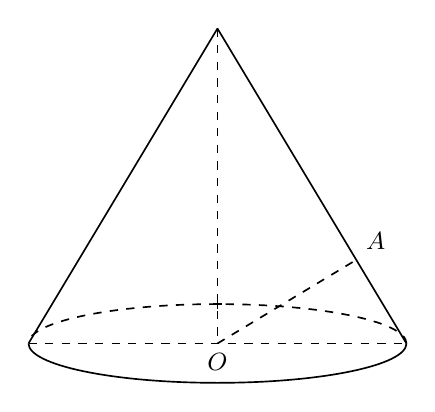
\begin{tikzpicture}[line width=0.6pt, font=\small]
  \coordinate (V) at (0,4);
  \coordinate (O) at (0,0);
  \coordinate (BL) at (-2.4,0);
  \coordinate (BR) at (2.4,0);
  \coordinate (A) at (1.76,1.06);
  % base ellipse: front solid, back dashed
  \draw (BL) arc [x radius=2.4, y radius=0.5, start angle=180, end angle=360];
  \draw[dashed] (BR) arc [x radius=2.4, y radius=0.5, start angle=0, end angle=180];
  % base diameter (hidden) dashed
  \draw[dashed] (BL) -- (BR);
  % axis (hidden) dashed
  \draw[dashed] (V) -- (O);
  % generatrices solid
  \draw (V) -- (BL);
  \draw (V) -- (BR);
  % OA dashed (foot of perpendicular from O to generatrix)
  \draw[dashed] (O) -- (A);
  % small cross where axis meets back arc
  \draw (0,0.5) ++(-0.06,0) -- ++(0.12,0);
  \draw (0,0.5) ++(0,-0.06) -- ++(0,0.12);
  % labels
  \node[below] at (O) {$O$};
  \node[above right] at (A) {$A$};
\end{tikzpicture}
